\subsection{Target}
This analysis probes the fundamental principles 
of Lorentz and CPT invariance. 
Recent theoretical breakthroughs have 
laid a foundation for experimental searches of 
quark-sector Lorentz- and CPT-violating
signatures in collider processes, including
the Drell-Yan process. The LHC provides unique
and ideal conditions for investigating 
much of this uncharted landscape.

Our target is to provide first results on Standard Model (SM)
quark-sector Lorentz- and CPT-violating effects from ATLAS 
measurements. Preliminary investigations 
suggest several first constraints on 
effects modifying the free propagation and
electromagnetic interaction vertex of the first
two quark generations will result from this target.

This analysis is planned as 
the first stage of a new search program 
studying sidereal oscillations of event observables, 
including the counting of $Z$ bosons 
in dilepton final states. Sidereal oscillations
are often described as ``smoking gun" signatures
of Lorentz and CPT violation. They arise from
violations of rotation invariance (recall 
that rotations form a subgroup of the Lorentz group). 
Most Lorentz- and CPT-violating effects produce sidereal oscillations.
Probing these signatures requires dedicated time-dependent
analyses involving the binning of measurements based on
when they were recorded.
As such, most prior works providing constraints
on Lorentz- and CPT-violating signatures
are indirect, phenomenological, and limited
to the smaller subset of time-independent
``rotation-invariant"
or ``boost-violating" signatures. 
A significant thrust of our program 
involves developing new methodologies
capable of capturing these 
comparatively numerous and challenging 
to directly access sidereal signatures. 

These latter methodologies are further motivated
by the fact that many previous studies 
have limited attention
to the renormalizable modifications and 
degrees of freedom that can be observed over long
durations (e.g. trapped electrons) 
or over large scales (e.g. cosmic microwave photons).
These modifications are mostly orthogonal 
to the leading signatures in collider processes
involving partons and electroweak bosons. 
The appearance of large collision energies coupled with 
nearly continuous event data is fertile 
ground for probing nonrenormalizable operators
of unstable or confined degrees of freedom 
and their associated higher-order sidereal signatures. 

While our focus here involves modifications of
the first two quark generations, it 
is crucial to emphasize that 
the heavy-quark, gluon, and 
$W^\pm$- and $Z$-boson sectors are also 
vastly unexplored. Upon completion 
of our target, we will extend our program to probe
new signatures associated to these sectors.

\subsection{Context}
\label{ssec:Context}
Lorentz invariance is a foundational assumption
of modern physics. It states that 
physical laws are independent of the relative orientation 
and velocity of an experiment in spacetime. 
For example, in the SM
Lorentz invariance applies 
globally (i.e. the same way at every spacetime point) 
and Lorentz transformations connect
observables from experiments rotated or boosted
relative to one another.
A deep consequence of this Lorentz invariance for
quantum field theories in flat spacetime
is the invariance of any process under
the combined operation of charge conjugation C,  
parity P, and time reversal T (CPT). This 
related discrete symmetry invariance 
follows from the CPT theorem.
%
When restricted to a local symmetry,
Lorentz invariance forms a core component 
of the Einstein equivalence principle 
underpinning General Relativity.
These strong theoretical motivations are accompanied by
numerous experimental results indicating 
Lorentz invariance holds over a wide
range of energies and systems \cite{datatables}.
Taken together, Lorentz invariance 
is among the most well-motivated guiding
principles in physics. 

Despite the numerous investigations undertaken to date, 
the Lorentz and CPT properties of some sectors of the SM, 
including the quark sector, remain virtually unexplored.
One reason for the comparatively few studies involving
quantum chromodynamics (QCD) degrees of freedom relative to
quantum electrodynamics (QED)---or, more generally, stable-particle 
degrees of freedom---is that, as in the conventional 
SM scenario, inferring quark-level 
properties from observables involving initial- and final-state hadrons 
is highly nontrivial. These technical complications 
persist when Lorentz and 
CPT invariance are relaxed. However, 
the theory STA members of this analysis, 
Enrico Lunghi and Nathaniel Sherrill, 
have resolved some of the basic issues on this front. 
They have constructed a Lorentz- and CPT-violating
extension of the leading-order (tree level) parton model
and have applied it to Drell-Yan dilepton production~\cite{Lunghi_2021}.
This analysis shows that a class of 
chiral quark-sector operators
challenging to isolate in other experiments 
can be studied in large momentum transfer $pp$ collisions where the 
participating quarks couple to $Z,W^{\pm}$ bosons.
The estimated size of these corrections are shown in 
Fig.~\ref{fig:coeff_bounds}. Details on the SME parameters
mentioned in the figure caption will be discussed in the following
Sec.~\ref{lab:Theory}.


\begin{figure}[htpb!]
\centering
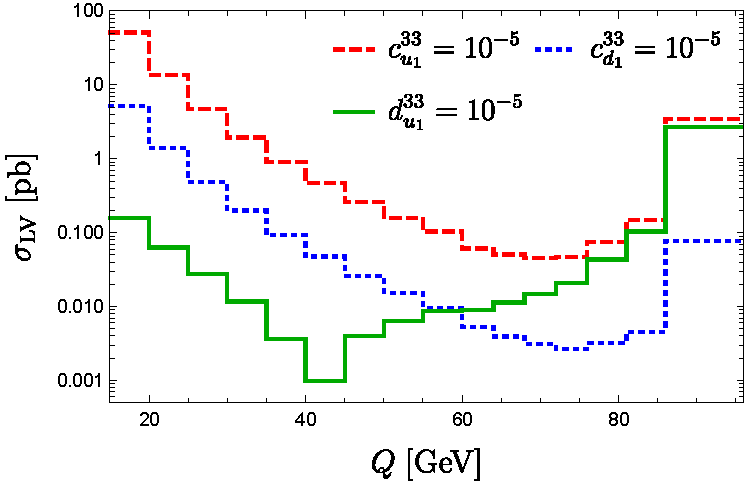
\includegraphics[scale=0.80]{figs/intro_theory/coeff_bounds.pdf}
\caption{
Order-of-magnitude estimates of sensitivity to laboratory
Standard-Model Extension (SME) coefficients as a function of $Q$ from predictions in 
Ref.~\cite{Lunghi_2021}. The $y$-axis
displays the Lorentz-violating contribution
to the total cross section in picobarns as
a function of invariant mass $Q$ from three
coefficients, $c_{u_1}^{33}, c_{d_1}^{33}$ and 
$d_{u_1}^{33}$ fixed to $10^{-5}$. 
The subscripts $u_1, d_1$ denote
the first-generation quarks, $u,d$. The superscripts
33 denote the 33-component of 
$c^{\mu\nu}_{u_1}$, etc. It is observed that the $c$-type coefficients
have most sensitivity to low $Q$ while the $d$-type
coefficient has most sensitivity on the $Z^0$ pole
at $Q = m_Z$. 
}
\label{fig:coeff_bounds}
\end{figure}
